\chapter{Methodology}
This chapter outlines the methodology employed to evaluate the effectiveness of an AI system based on MARQ in solving mind sports with imperfect information. The approach involves the development of a competitive system, followed by the evaluation of its performance through win-rate analysis against human players and an assessment of its adaptability across diverse game environments. The subsequent sections detail the processes and methods that will be used to achieve these research objectives.

\section{Project Planning}
This research will be conducted according to a structured plan encompassing participant selection, sample size determination, and experimental procedures. The project will follow a rapid prototyping approach for the design and implementation of the AI system. The timeline is segmented into four distinct phases. The development phase will run from September 2025 to February 2026, beginning with game environment development from September through November 2025, followed by AI training from December 2025 to January 2026, and concluding with system deployment in February 2026. The user testing phase will take place in March 2026, involving one-on-one matches and data collection activities. The final analysis and documentation phase will commence in April 2026, focusing on data analysis and manuscript preparation.

\subsection{Community Introduction to Stratego}
The introduction of the game Stratego to the participant community is a prerequisite for this study. This necessity arises from a complete lack of available local participants possessing prior knowledge of the game's rules or strategies. Unlike more popular games like Chess, Stratego's niche status means a pre-existing pool of experienced players is not available for participation to test against MARQ. Therefore, a structured introduction is essential to cultivate the necessary participant cohort from the ground up. This approach ensures all participants begin with a uniform baseline understanding. It allows for the parallel development of both human expertise and artificial intelligence, creating a synchronized learning environment where the adaptive capabilities of the MARQ system can be fairly assessed against a human cohort that is also in the process of learning.

\subsection{Participant Selection}
The participant selection process is designed to recruit a cohort of 20 individuals via convenience sampling, taking into account the project's resource constraints while still yielding a enough sample. The target demographic is enthusiasts of strategic mind sports of a diverse age and game experience.

Prospective participants will be screened to evaluate two key attributes. Their strategic game experience is key to ensuring a baseline aptitude, and second, their confirmed lack of prior knowledge of Stratego to ensure the study's "synchronized learning" premise. Ultimately, only those who successfully finish the screening phase will be admitted, guaranteeing they possess the necessary foundational skills to provide meaningful interaction with the MARQ system and substantive feedback.

\subsection{Experimental Procedures}
One-on-one matches between human participants and the MARQ system will be conducted on-site using a single device. To ensure consistency, each participant will receive a checklist outlining the procedures for interacting with the game.

Each session will last one (1) hour, during which participants must complete at least two (2) games against MARQ. Additional games may be played if the time permits. The following game statistics will be recorded will include the winner, total game duration, total moves per player, and the number and type of remaining pieces for both players. Immediately following the session, each participant will be given an evaluation form to provide open-ended feedback on their experience.

\section{System Development}
The system development consists of two components which is the game environment and MARQ. The game environment will be developed to serve as the interface for human players and the world in which the AI agent operates. While MARQ is the trained model to be used as the bot playing against the player.

\subsection{Piece Value Computation}
To inform MARQ's reward function and internal heuristics, a quantitative value was assigned to each piece in Stratego. This was achieved through a systematic process to account for the relative power of each piece.
\begin{enumerate}
\item {Initial Unweighted Calculation:} The value of each piece was first computed using the formula:
\[
\text{Unweighted Piece Value} = a - b
\]

where a is the number of pieces it defeats and b is the number of pieces it loses to.
\item {Normalization:} The computed values were then normalized to a range of [0,1] using min-max scaling to create a standardized set of weights, typically used in chess evaluation.
\item {Final Weighted Calculation:} The final value was then recomputed by weighting each interaction:
\[
\text{Final Piece Value} = \sum_{i \in \text{beats}} w_i \;-\; \sum_{j \in \text{loses to}} w_j
\]
\end{enumerate}
 
where \(w_i\) and where \(w_j\) are the normalized values of the pieces it beats or loses to, respectively. This provides a more accurate reflection of each piece's strategic importance.

\subsection{Handling Imperfect Information: Probabilistic Belief State (PBS)}
A key challenge in Stratego is the unknown identity of opponent pieces. To address this, the MARQ system will incorporate a Probabilistic Belief State (PBS). The PBS is a matrix that maintains a probability distribution for the identity of each of the opponent's unrevealed pieces. This belief state is updated throughout the game using two forms of reasoning:
\begin{itemize}
\item {Deductive Reasoning:} When a piece interaction occurs, the PBS is updated with absolute certainty. The probabilities of the unknown piece being a Scout, Miner, or Sergeant would be set to 0, and the remaining probabilities are renormalized.
\item {Inductive Reasoning:} The system infers piece identity from an opponent's behavior. For example, a piece that moves frequently and far is more likely to be a Scout. A piece that moves away from a threat exhibits defensive behavior, slightly increasing the probability that it is a high-value piece like the Flag or Marshal. These behavioral heuristics, based on aggression, defensiveness, and movement patterns, are used to adjust the probabilities in the PBS via Bayesian updates.

\item {Real state vs. PBS comparison:} The system compares the  PBS with the real state of the board and can be updated to allign more to the true piece for training. Training will have two stages separated, creating the belief state and later on normalizing the values from the real state to the PBS for a more accurate prediction. The main purpose of the PBS is to create a pseudo-perfect information game out of the imperfect information.
\end{itemize}

\section{Model Training}
The most time-intensive part of the research. Mainly due to the computation needed by the model to learn both exploration and exploitation. Since we are using a DQN model, the epsilon value in the first few games will be large, making the model have a higher likelihood of choosing random moves to try and explore. Once the epsilon value becomes smaller and smaller the model tends to follow what it thinks will be the optimal move.

The state representation provided to the DQN is crucial. It will be a multi-channel tensor including: (1) the location of the player's pieces, (2) the location of known opponent pieces, and (3) the complete Probabilistic Belief State (PBS) for all unknown pieces. 

Every 100 episodes, the target model or history model will be synced from the policy network, along with the memory replay by the AAREN.

\begin{figure}[htbp]
\centering
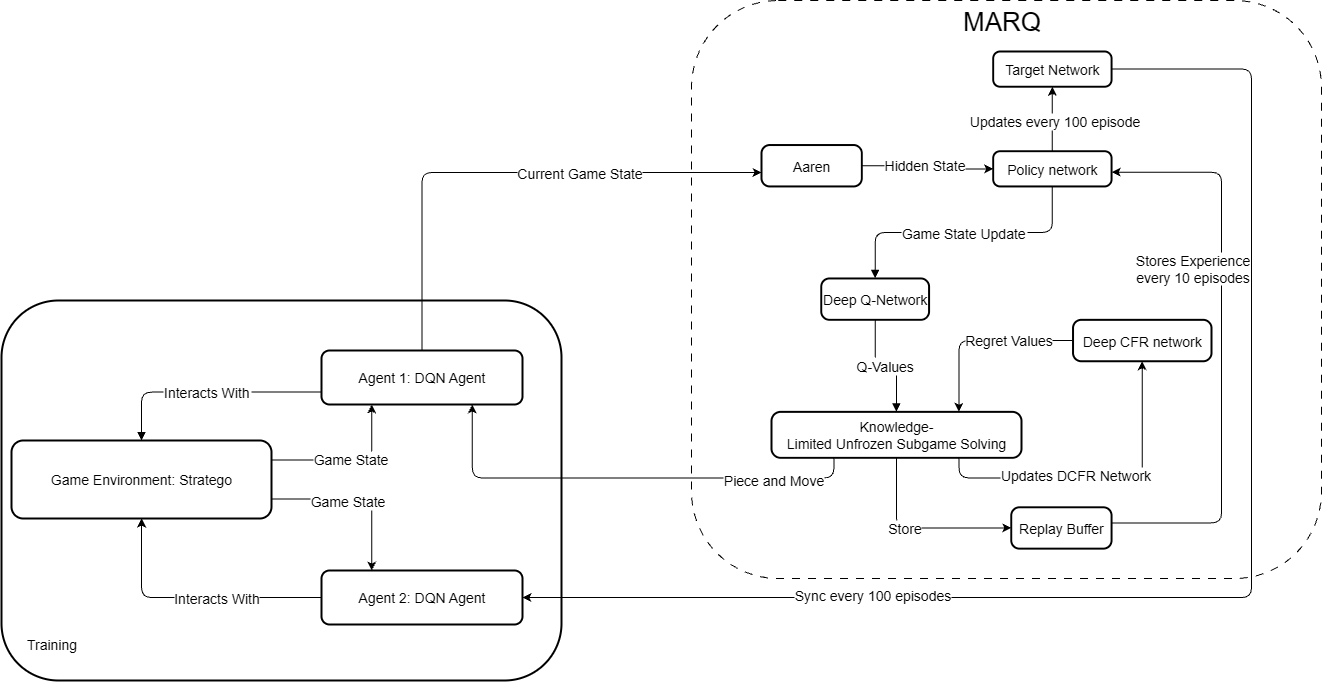
\includegraphics[width=1\textwidth]{figures/DQN Architecture.png}
\caption[MARQ Framework]{The MARQ System Architecture, which takes the Board State and PBS as input.}
\label{fig:my_label}
\end{figure}


\subsection{Deployment}
Upon completion of the training and validation cycles, the best-performing MARQ model weights will be saved and finalized for deployment. Deploy the trained model into the Stratego game environment described in Section 2 of the methodology.

The deployed system will function as the complete application used during the user testing phase. It will be configured to run locally on the single device designated for the experimental procedures. In this production mode, the model's exploratory functions will be deactivated for a more measured approach from the agent, always selecting the action with the highest predicted Q-value. This ensures that all human participants compete against the identical, optimized version of the MARQ AI, providing a consistent baseline for the quantitative and qualitative evaluations.

\begin{figure}[ht]
    \centering
    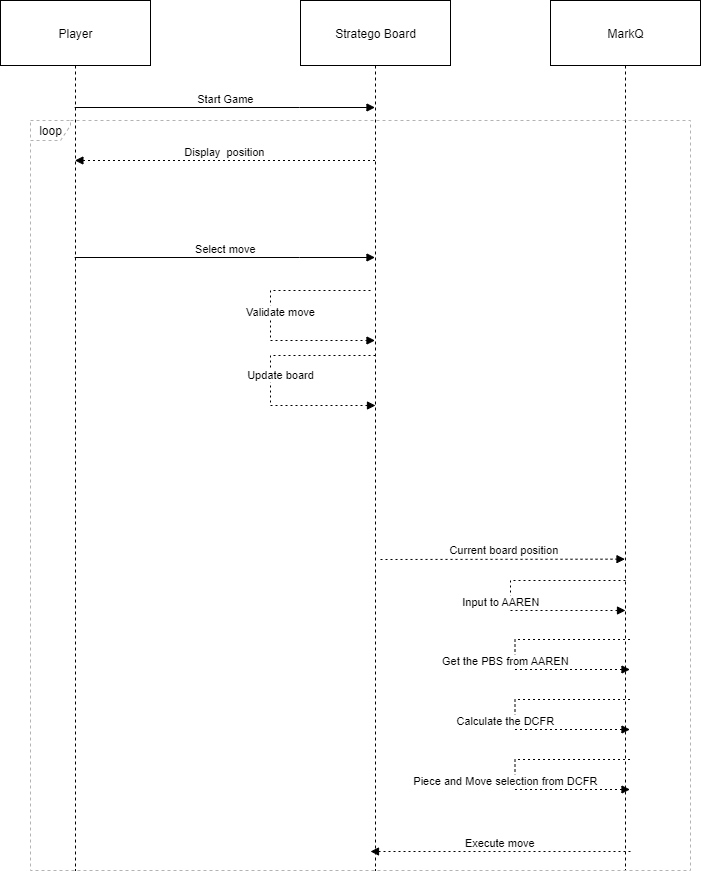
\includegraphics[width=.5\textwidth]{figures/Game diagram.png}
    \caption{Game Sequence Diagram}
    \label{fig:Sequence Diagram}
\end{figure}

In the figure above, the player starts the game and the loop begins until either the player wins by getting the flag of the agent or loses if the agent reaches the player's flag. The agent gets the current position and sends it to AAREN, constructing the possible positions of the board. After getting the PBS, it is then used to calculate the possible moves and actions that can be taken by the DeepCFR. Once the DeepCFR calculates pieces that are possible to have moves, it is then the role of the DQN to formalize a strategy to be used. 
\section{Evaluation}
A comprehensive evaluation approach combining quantitative and qualitative methods will be used to assess the MARQ system's performance and the user experience.

\subsection{Quantitative Analysis}
The quantitative assessment of the model's performance is conducted through the Evaluation component. Key metrics are tracked to gauge learning progress and strategic capability. Primary analytics include:
\begin{itemize}
\item {Win Rate\%}: The percentage of games won against human participants.
\item {Average Game Length}: The mean number of moves or duration of games, indicating game efficiency.
\item {Decision-Making Speed}: The average time taken by the agent to select an action.
\item {Loss Curves}: The progression of policy and value loss over training time, indicating the stability of the learning process.
\item {Player Performance over Time}: To evaluate the "synchronized learning" environment, a two-tailed paired t-test will be used. This will determine if there is a statistically significant difference in gameplay metrics (e.g., difference in remaining pieces) between a player's first and last games, assessing if human players improve against the AI.

The results from the Likert-scale questions will be analyzed using a weighted mean to derive a quantitative score for each dimension of user acceptance.
\end{itemize}

\subsection{Qualitative Analysis}
To assess the end-user opinion on usability, a usability testing session will focus on gathering participant feedback through an evaluation form. The form will evaluate three key dimensions:
\begin{itemize}
\item {Performance:} Assessing the agent's speed, consistency, and perceived strategic competence.
\item {Usability:} Evaluating the ease of use, intuitiveness of the interface, and overall user experience.
\item {Relevance:} Gauging the AI's value as a strategic tool and its potential for helping players learn Stratego.
\end{itemize}


\subsection{Model Version History}
The development of MARQ is an iterative process. Each model version represents a snapshot of this evolution, performance metrics, and reliability. 

\subsection{Initial Training}

Under Appendix B are the initial training results of 1000 training cycles or episodes. We can see that the early training phase is not yet refined due to the agent being in the exploratory phase, ready to search and find an exploitable strategy. The reward indicates that it is having a hard time finding a good strategy to fight against the other agent. The win-rate stayed to a draw due to the agents being on an endless loop of moving pieces back in forth. Another issue is that the agent has reduced epsilon, making the moves deterministic, and only picking the "best move" with the highest q-value. 
